\section{Experiments}
\seclabel{experiments}

\TODO{Update results with any experiments. The current section basically reflects what we should expect but I'm running a few with slightly more test objects to see what happens}

We evaluate the convergence rate of the Dex-Net 1.0 algorithm for varying sizes of prior data used from Dex-Net and explore the sensitivity of the convergence rate to object shape, the similarity kernel bandwidths, and uncertainty.
We created two training sets of 1000, and 10000 objects by uniformly sampling objects from Dex-Net.
From the remaining objects, we created a set of 300 validation objects for selecting algorithm hyperparameters and a set of 45 test objects.
We ran our algorithm with $N_n = 10$ nearest neighbors and used isotropic uncertainty with object and gripper translation variance $\sigma_{t} = 0.005$, object and gripper rotation variance $\sigma_{r} = 0.1$, and friction variance $\sigma_{\gamma} = 0.1$.

The bandwidths of our similarity kernel were constrained to be diagonal for the grasp parameters features $C_g = \Lambda$, isotropic for the global shape features $C_s = \sigma I$ for $\sigma \in \bR$, and a Gaussian mask $C_d$ centered on the differential heightmaps with height $w_d \in \bR$ and variance $\sigma_d \in \bR$.
The bandwidths were selected by maximizing the log likelihood of the true $P_F$ under the CCBP model on the validation set using a grid search over hyperparameters.

To scale the experiments, we developed a Cloud-based software library on top of Google Cloud Platform.
We used Google Compute Engine (GCE) to distribute trials of MAB algorithms across objects and Google Cloud Storage to store Dex-Net.
Our experimental scripts launched up to 1500 GCE single core instances at one time for hyperparameter tuning and convergence analysis, reducing the runtime of our experiments by over $1000\times$.

\subsection{Scaling of Average Convergence Rate}

To examine the effects of orders of magnitude of prior data on convergence to a grasp with high $P_F$, we ran Algorithm~\ref{alg:full} on the 20 validation objects with priors computed from 1,000 and 10,000 objects from Dex-Net. 
~\figref{avg-reward} shows the normalized $P_F$ (the ratio of the $P_F$ for the sampled grasp to the highest $P_F$ of the 250 candidate grasps) versus iteration averaged over 25 trials for each of the 20 validation objects for 4,000 iterations.
The plot also compares Algorithm~\ref{alg:full} to uncorrelated Thompson sampling and uniform allocation~\cite{laskey2015bandits}.
Our algorithm with 10,000 objects takes approximately $3.5\times$ fewer iterations to reach the maximum normalized $P_F$ value reached by Thompson sampling over all iterations.
Furthermore, the 10,000 object curve does not fall below 90\% of the best grasp in the set across all iterations, suggesting that a grasp with high $P_F$ is found using prior data alone.
%However, we see that on average our algorithm makes progress more slowly than Thompson sampling.

\begin{figure}[t!]
\centering
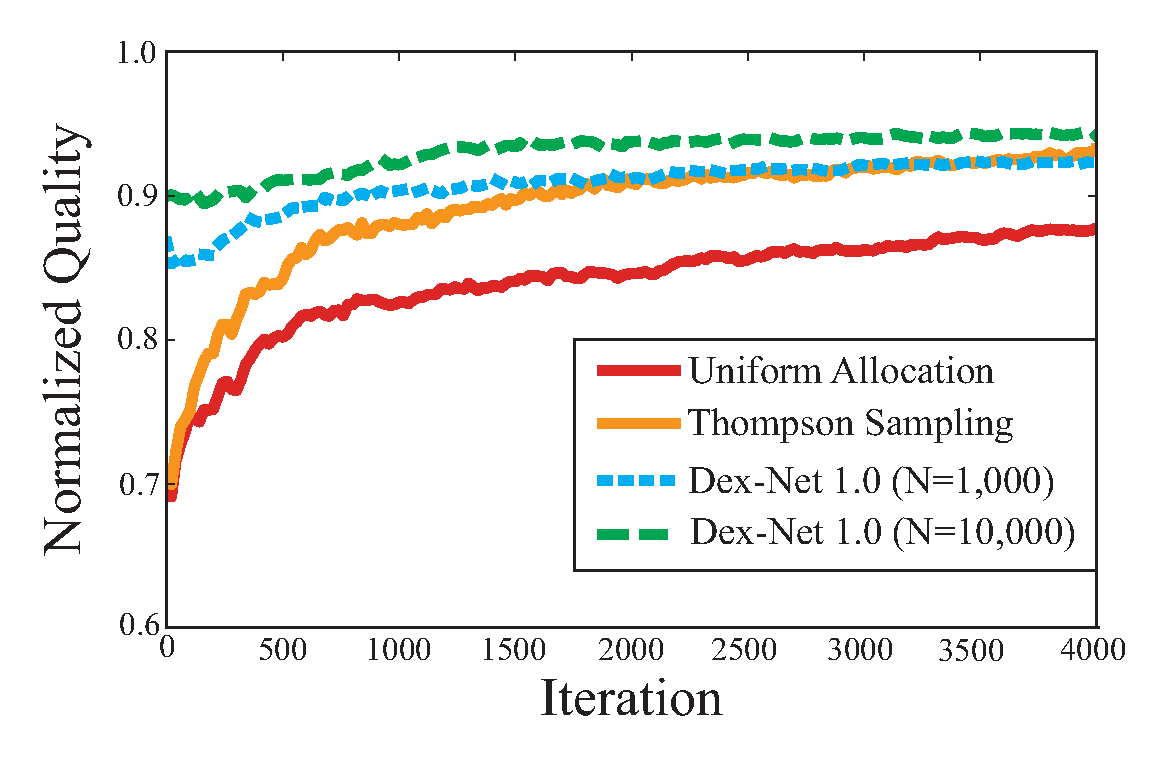
\includegraphics[scale=0.45]{figures/illustrations/avg_reward.eps}
\caption{Average normalized grasp quality versus iteration over 20 validation objects and 25 trials per object for our algorithm with 1,000 and 10,000 prior 3D objects from Dex-Net. We measure quality by the $P_F$ for the best grasp predicted by the algorithm on each iteration and compare with uncorrelated Thompson sampling and uniform allocation. We see that our algorithm converges faster with 10,000 models, never dropping below approximately 90\% of the grasp with highest $P_F$ from the 250 candidate set.}
\figlabel{avg-reward}
\vspace*{-15pt}
\end{figure}

\subsection{Sensitivity to Object Shape}
\seclabel{shape-sens}
To understand the behavior of Algorithm~\ref{alg:full} on individual 3D objects, we examined the convergnce rate with a 3D model of the only drill in Dex-Net and a spray bottle, which is an uncommon object category but has a few examples in Dex-Net.
~\figref{avg-reward-obj} shows the normalized $P_F$ (the ratio of the $P_F$ for the sampled grasp to the highest $P_F$ of the 250 candidate grasps) versus iteration averaged over 25 trials for 4,000 iterations on these two objects.
We see that the spray bottle converges very quickly when using a prior dataset of 10,000 objects, finding the optimal grasp in the set in about 1,500 iterations.
\figref{spray-grasps} illustrates the grasps predicted to have the highest $P_F$ on the spray bottle by the different algorithms after 100 iterations.
However, performance on the drill does not increase using either 1,000 or 10,000 objects.

This suggests the value of the Dex-Net objects found by our shape similiarty MV-CNN, displayed in \figref{query}.
We see that the spray bottle has no nearest neighbors that are very close in shape in the 1,000 object dataset, but in the 10,000 object dataset two nearly identical spray bottles are retrieved.
On the other hand, the drill has no similar neighbors in either dataset, and the closest model in all of Dex-Net according to our similarity metric is a phone.

\begin{figure}[t!]
\centering
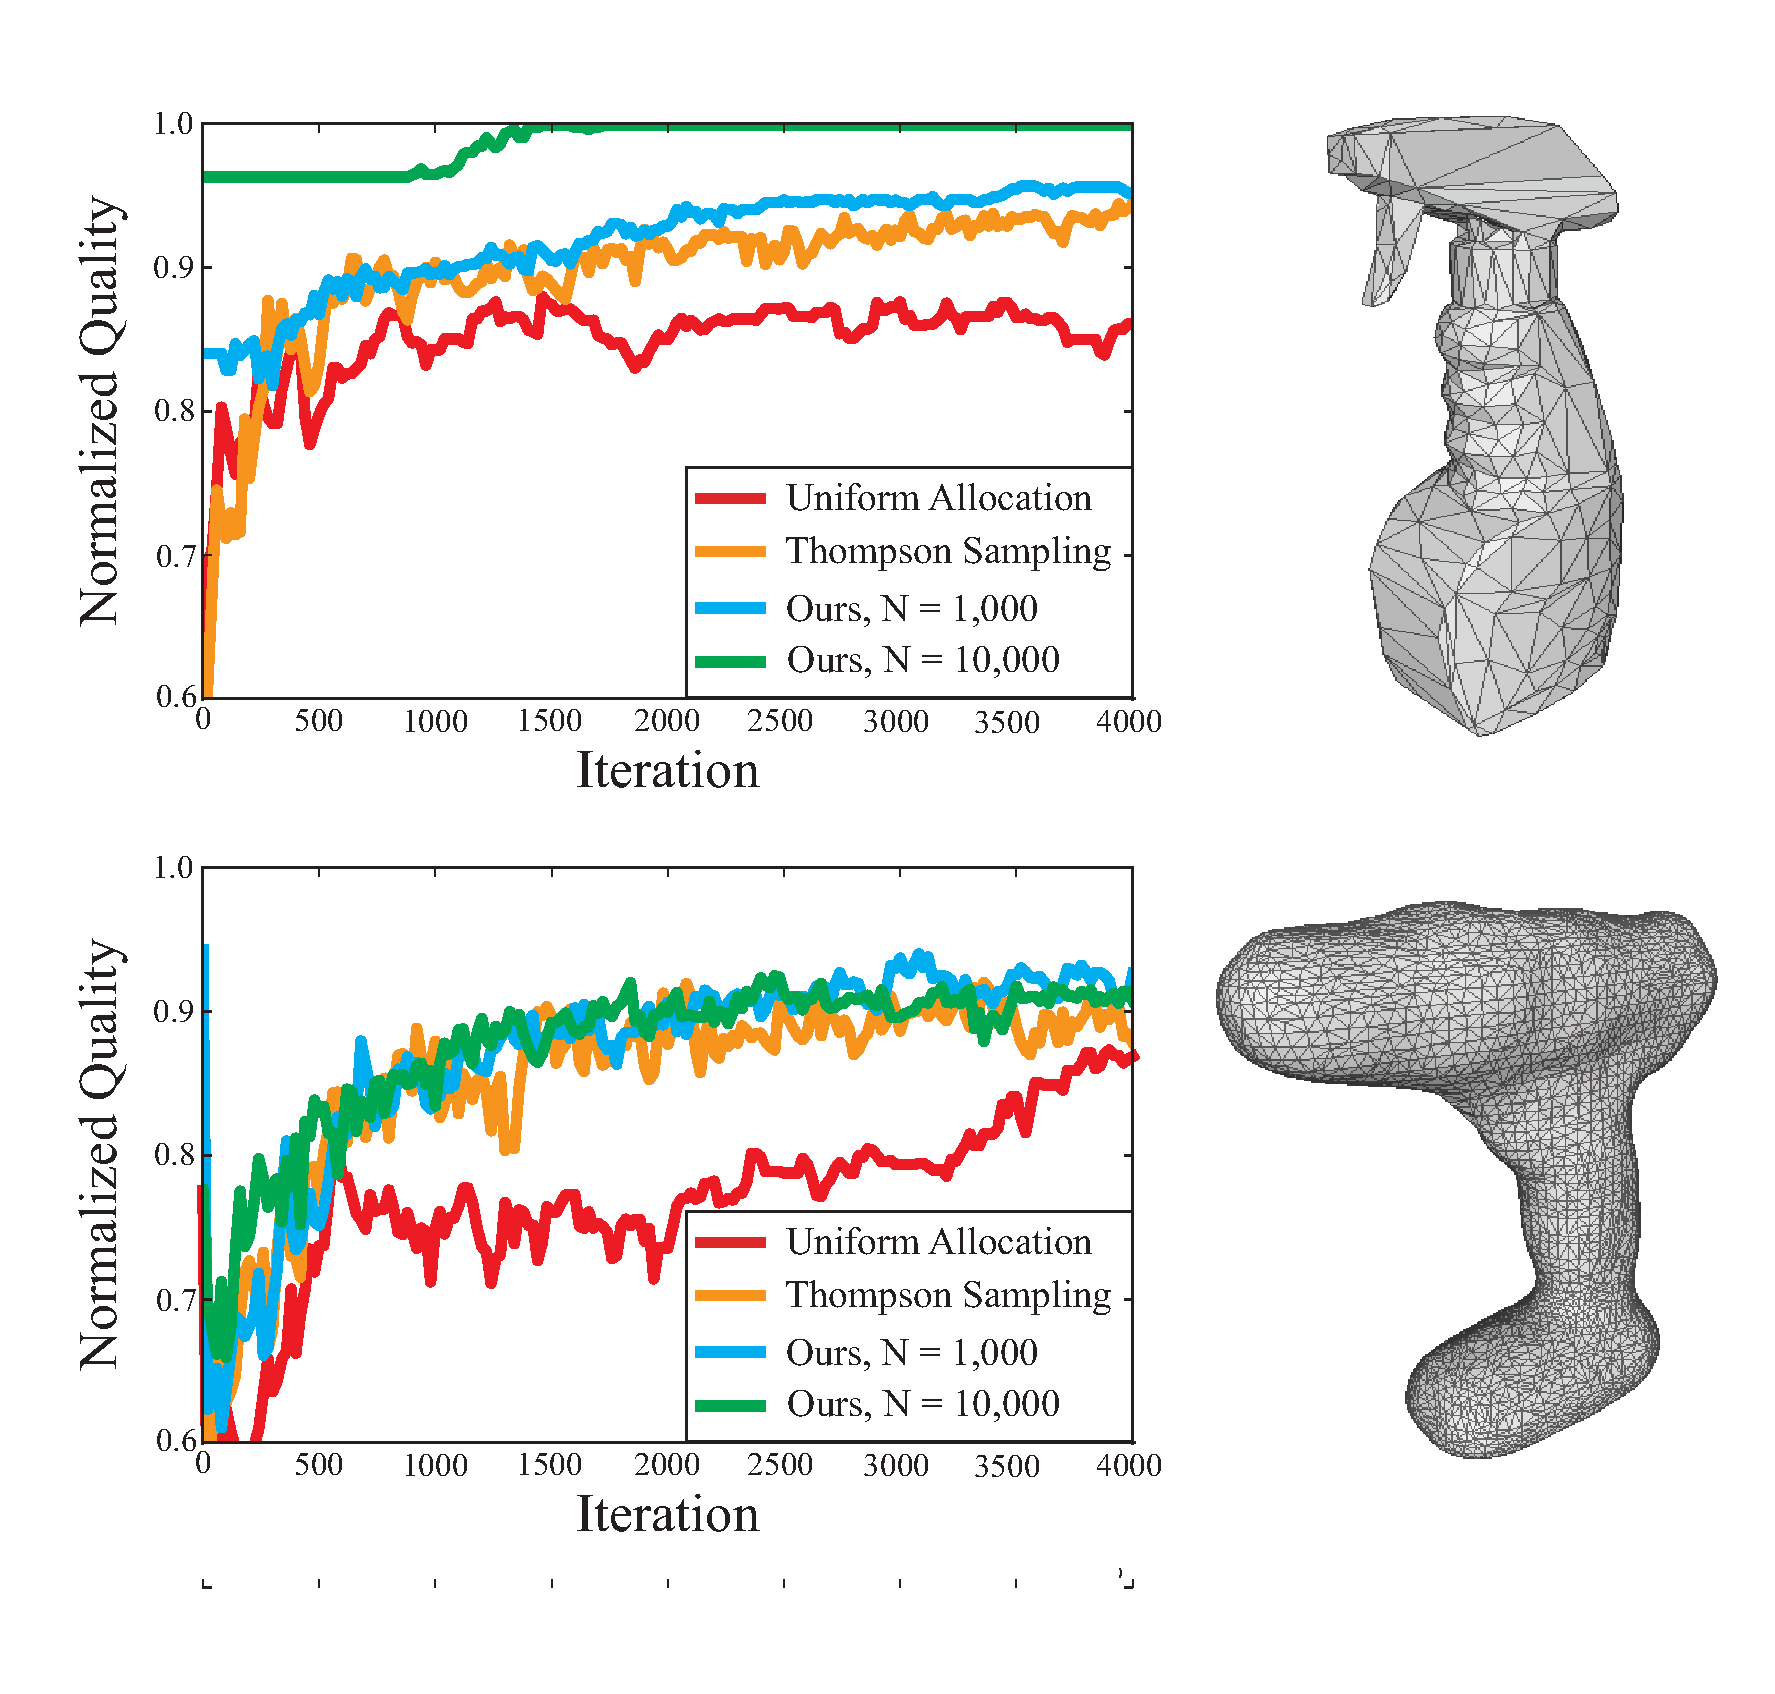
\includegraphics[scale=0.31]{figures/illustrations/avg_reward_drill.eps}
\caption{Average normalized grasp quality versus iteration over 25 trials per object for our algorithm with 1,000 and 10,000 prior 3D objects from Dex-Net on a spray bottle (top) and drill (bottom). We measure quality by the $P_F$ for the best grasp predicted by the algorithm on each iteration and compare with uncorrelated Thompson sampling and uniform allocation. (Top) For the spray bottle, Algorithm~\ref{alg:full} does not outperform Thompson sampling for 1,000 objects, but quickly converges to the optimial grasp once 10,000 objects are used. (Bottom) The drill, which is relatively rare in the dataset, has no noticeable performance increase over Thompson sampling, even with 10,000 objects.}
\figlabel{avg-reward-obj}
\vspace*{-15pt}
\end{figure}

\begin{figure}[t!]
\centering
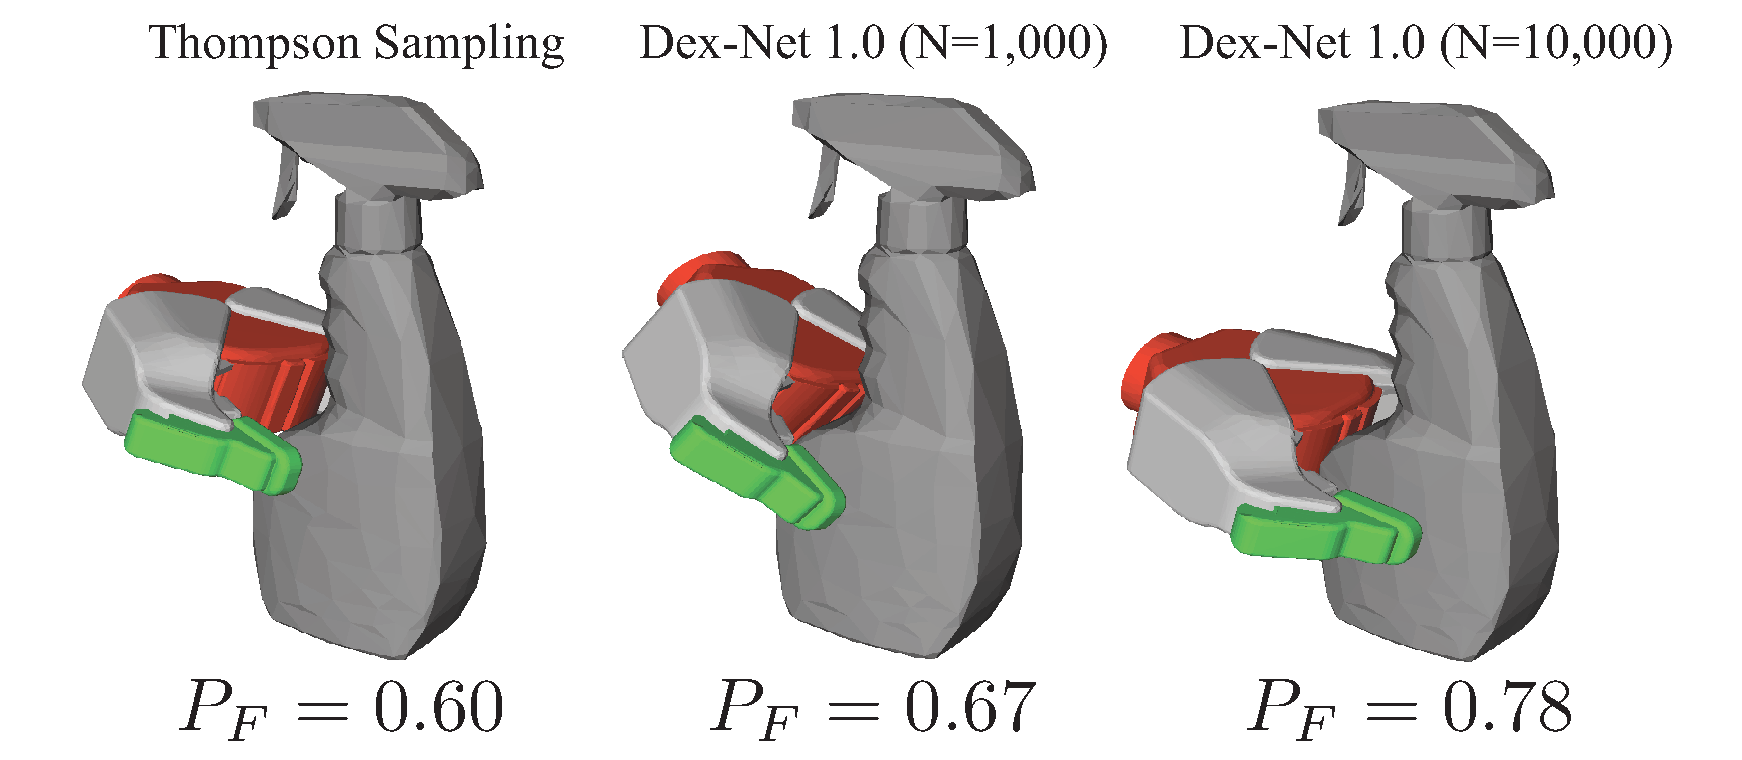
\includegraphics[scale=0.28]{figures/illustrations/spray_grasps.eps}
\caption{Illustation of the grasps predicted to have the highest $P_F$ after only 100 iterations by Thompson sampling, Algorithm~\ref{alg:full} with 1,000 prior objects from Dex-Net, and Algorithm~\ref{alg:full} with 10,000 prior objects from Dex-Net. Thompson sampling chooses a grasp near the edge of the object, while our algorithm selects grasps closer to the center-of-mass of the object.}
\figlabel{spray-grasps}
\vspace*{-5pt}
\end{figure}

\begin{figure}[t!]
\centering
\includegraphics[scale=0.38]{figures/illustrations/nearest_neighbors.eps}
\caption{Illustration of the five nearest neighbor objects from Dex-Net to the spray bottle and drill using the multi-view CNN-based shape embedding and Euclidean distance for size 1,000 and 10,000 datasets from Dex-Net. We see that for the 1,000 object dataset neither model has relevant neighbors, while for the 10,000 object dataset two other spray bottles are returned. However, even with 10,000 objects no object geometrically similar to the drill is found. }
\figlabel{query}
\vspace*{-5pt}
\end{figure}

\section{Sensitivity to Similarity Kernel Bandwidth}
\seclabel{band-sens}
We also studied the sensitivity of our algorithm to the kernel bandwidth hyperparameters described in \secref{ccbps}.
We varied the bandwidth of the kernel for the heightmap gradients to the higher value $1 / 350$ and the lower value $1 / 450$ , as this was the most discriminative feature maps found by our hyperparameter tuning.
\figref{bandwidth-sens} shows the normalized $P_F$ versus iteration averaged over 25 trials for 4,000 iterations on the 20 validation objects.
We see that increasing the bandwidth of the kernel can reduce performance to be on par with uniform allocation.
This may be because overestimating similarities can lead to a grasp with high $P_F$ being predicted too low, or vice versa.
One the other hand, decreasing the bandwidth also decreases the convergence rate but Algorithm~\ref{alg:full} with 10,000 prior objects still outperforms Thompson sampling.
This suggests that a conservative setting of similiarity kernel bandwidth is important.

\begin{figure}[t!]
\centering
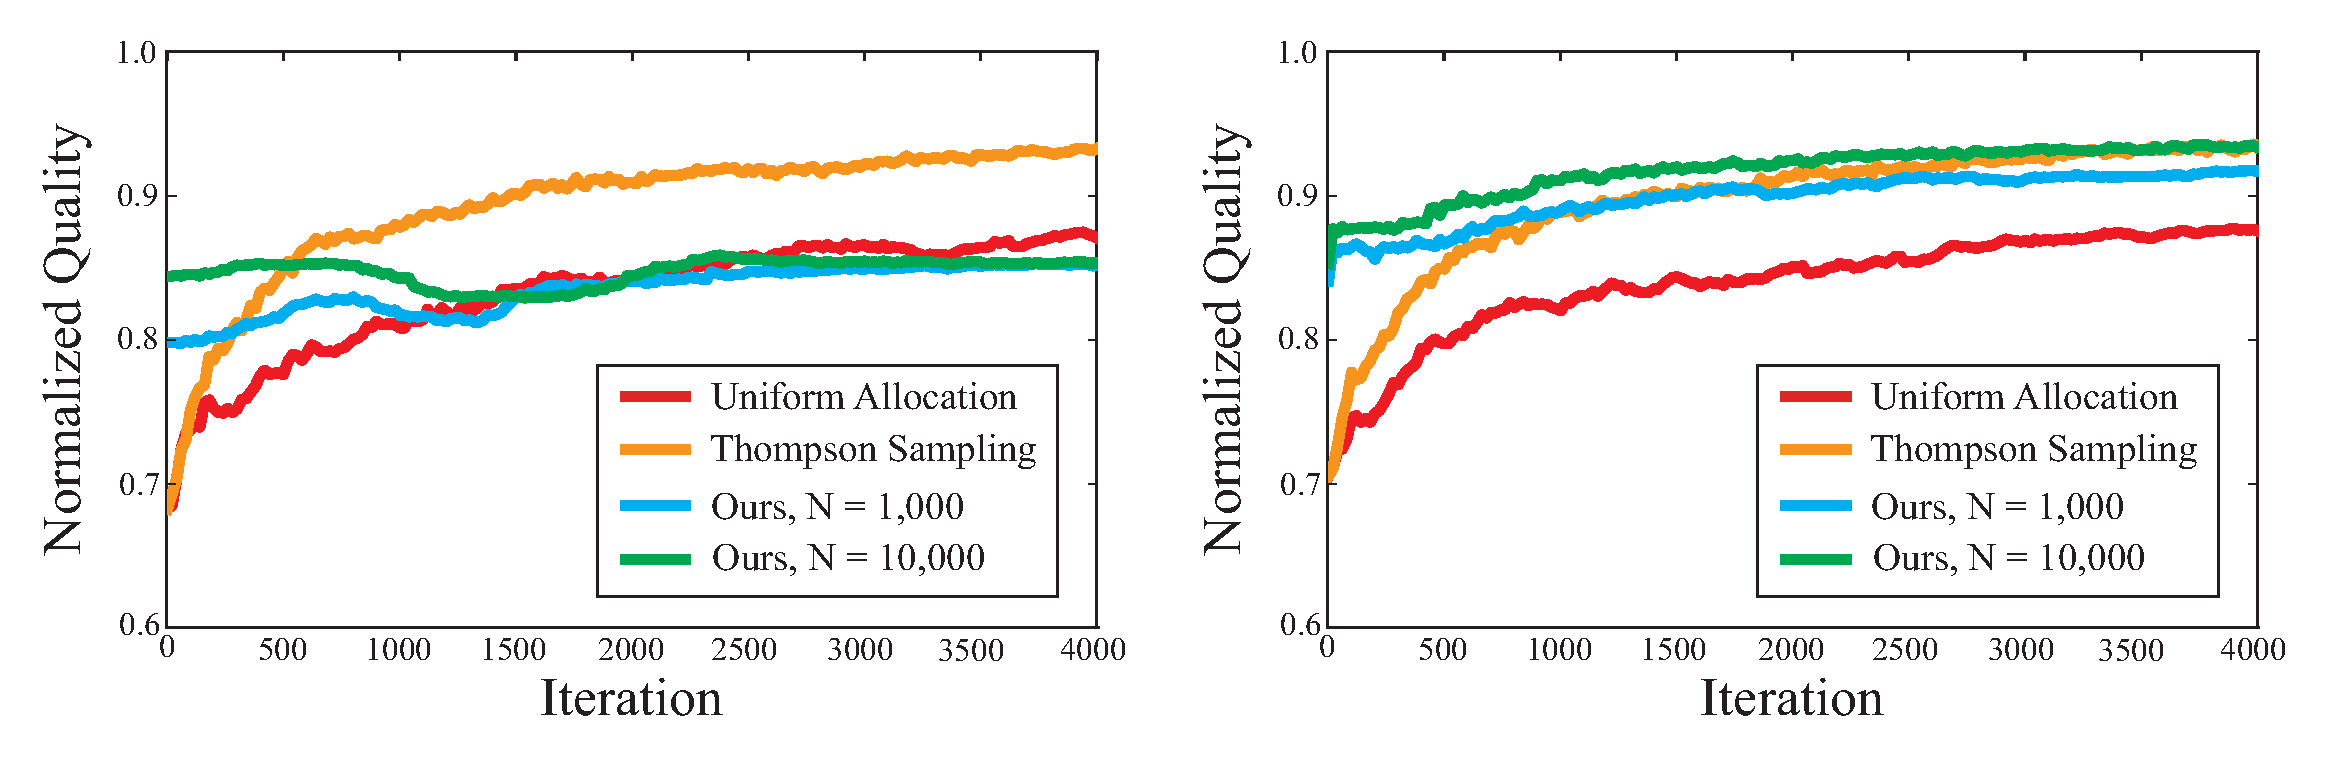
\includegraphics[scale=0.23]{figures/illustrations/weight_sensitivity.eps}
\caption{Average normalized grasp quality versus iteration over 25 trials per object for our algorithm with 1,000 and 10,000 prior 3D objects from Dex-Net with a higher heightmap gradient kernel bandwidth of $1 / 350$ (left) and a lower kernel bandwidth of $1 / 450$ (right). (Left) Using a higher kernel bandwidth causes the algorithm to measure false similarities between grasps, leading to performance on par with uniform allocation. (Bottom) A lower kernel bandwith decreases the convergence rate, but Algorithm~\ref{alg:full} still selects a grasp within 85\% of the grasp with highest $P_F$ for all iterations, on average.}
\figlabel{bandwidth-sens}
\vspace*{-10pt}
\end{figure}

\section{Sensitivity to Pose and Friction Uncertainty}
\seclabel{u-sens}
We also studied the sensitivity of our algorithm to the levels of object pose, gripper pose, and friction coefficient uncertainty for the test object.
We tested low uncertainty with object and gripper translation variance $\sigma_{t} = 0.0025$, object and gripper rotation variance $\sigma_{r} = 0.05$, and friction variance $\sigma_{\gamma} = 0.05$ as well as high variance $\sigma_{t} = 0.01, \sigma_{r} = 0.2,$ and $\sigma_{\gamma} = 0.2$.
The uncertainty levels used to label grasps in Dex-Net were not changed.
\figref{u-sens} shows the normalized $P_F$ versus iteration averaged over 25 trials for 4,000 iterations on the 45 test objects.
The normalized $P_F$ for increases and descreases across all methods for low and high uncertainty, respectively.
Also, prior data no longer increases convergence rate but a mismatch between the uncertainty on the test object and training objects does not cause performance to decrease below Thompson sampling without priors.

\begin{figure}[t!]
\centering
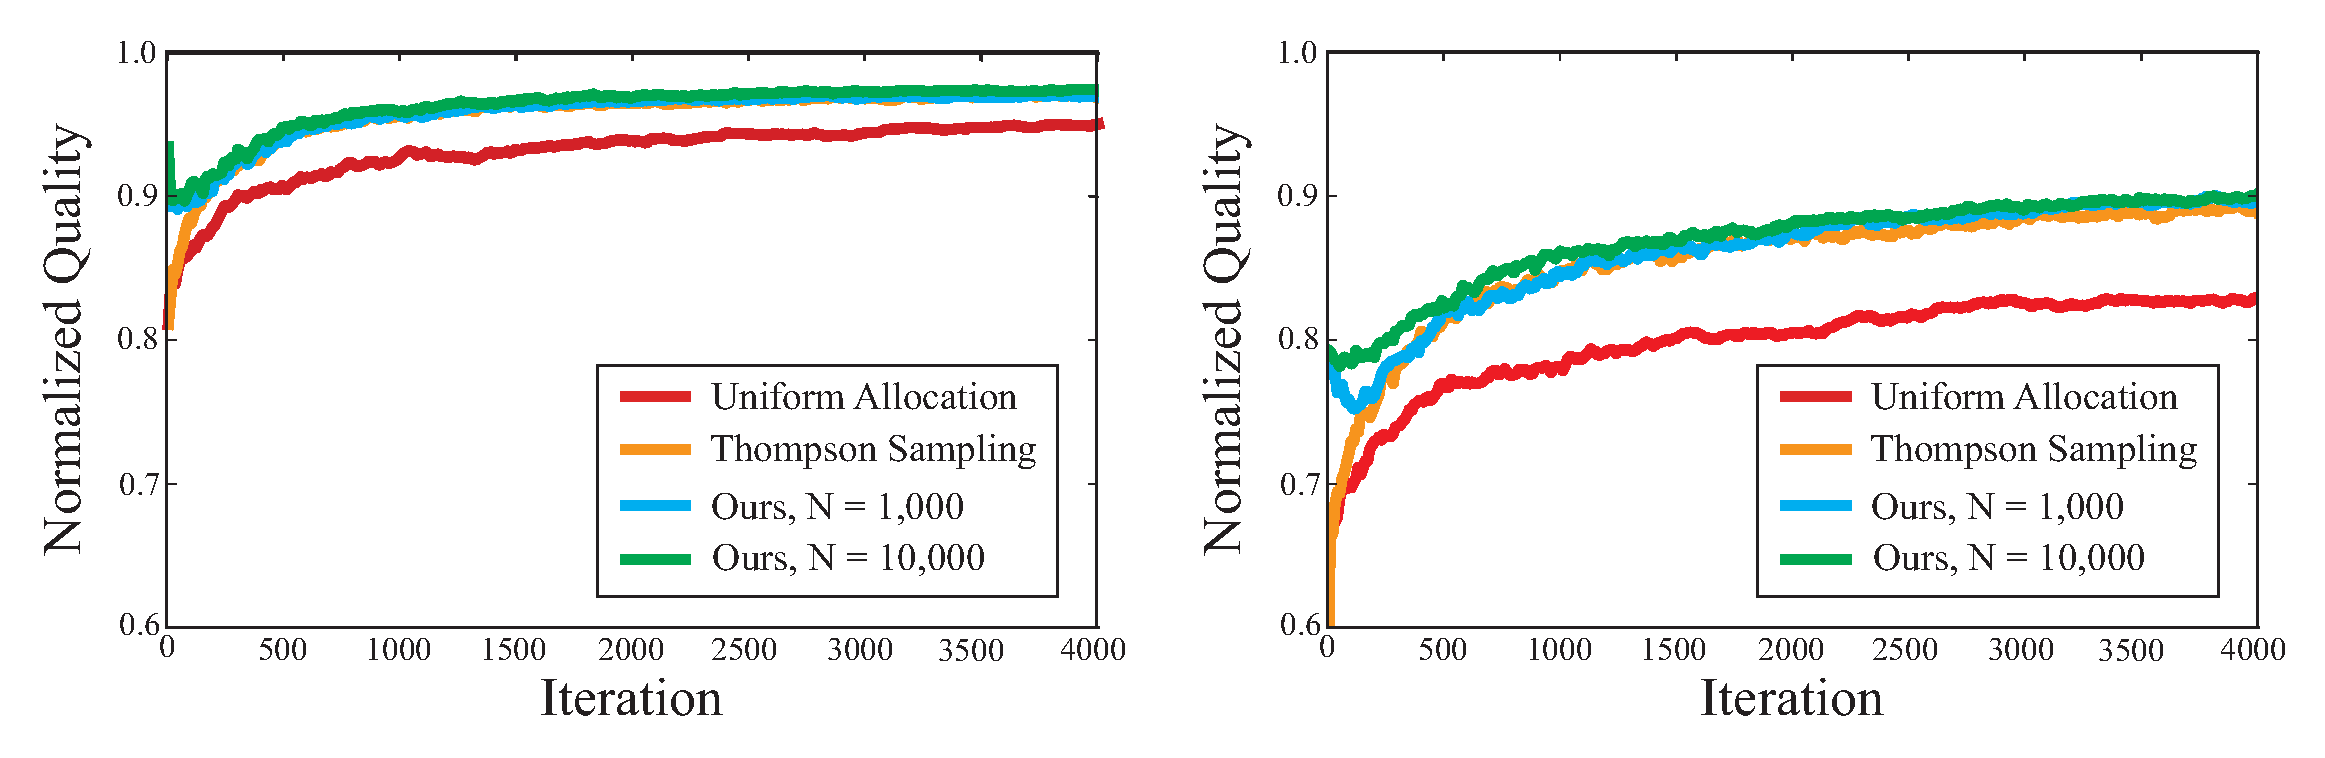
\includegraphics[scale=0.23]{figures/illustrations/u_sensitivity.eps}
\caption{Average normalized grasp quality versus iteration over 25 trials per object for our algorithm with 1,000 and 10,000 prior 3D objects from Dex-Net with low uncertainty (left) $\sigma_{t} = 0.0025, \sigma_{r} = 0.05, \sigma_{\gamma} = 0.05$ and high uncertainty (right) $\sigma_{t} = 0.01, \sigma_{r} = 0.2, \sigma_{\gamma} = 0.2$ on the test set. Lower uncertainty increases the quality for all methods and higher uncertainty decreases the quality for all methods. Interestingly, in both cases prior data has little effect but the convergence rate is still on par with Thompson sampling with no prior data.}
\figlabel{u-sens}
\vspace*{-10pt}
\end{figure}
